\chapter*{Executive Summary}
The shortage of \iso[3]{He} has caused the Domestic Nuclear Detection Office (DNDO) within the U.S. Department of Homeland Security (DHS) to sponsor research for alternative radiation portal monitors (RPM).
The DNDO/DHS in conjunction with Pacific Northwest National Lab (PNNL) have established performance criteria that replacement technologies must satisfy.
Replacement technologies must fulfill three basic criteria: 1) a neutron detection efficiency, 2) a gamma insensitivity, and 3) the performance of the detector should not suffer in the presence of a strong gamma field.
Polymeric films containing \iso[6]{Li} ranging from 15 to 300 microns have the ability to fulfill these criteria if suitably utilized.
For a typical detector this involves maximizing the neutron-gamma discrimination, maximizing the physical detector configuration in order to ensure optimal use of the incident neutron spectra, and ensuring that the scintillation light generated can be collected.

A pulse height discriminator for rejecting gamma interactions has been determined for polymeric films ranging from 15 microns to 300 microns in thickness. 
The ability for this pulse height discriminator has been investigated and attributed to the energy deposition in the material by the reaction products of the gammas and neutrons, where the Compton scattered electrons from a photon interaction generally have energies in the hundreds of keV while the \iso[6]{Li} reaction products have energies in the 10 keV range. 
Detailed GEANT4 simulations indicate that a desired film thickness is around 100 microns. 

A replacement portal monitor has then been designed for layered polymeric films that effectively utilize the \iso[6]{Li} in the detector material. 
These layered detector designs consist of thin film layers sandwiched between a light guide, in this case a wavelength shifter.
A genetic algorithm was employed to optimize the interaction rate above the necessary discriminator level for three different types of detector materials.
Two of these materials were composite polymers developed at the University of Tennessee, consisting of a polystyrene based film and a polyethylene naphthalene film.
The third material was a commercial scintillator, \iso[6]{LiF} loaded ZnS:Ag (EJ-426HD).
An example of the an optimized geometry is shown in \autoref{fig:EXSumDemoLiFZnS} in which the films are \SI{100}{\um} placed in a wavelength shifter.
\begin{figure}
  \centering
  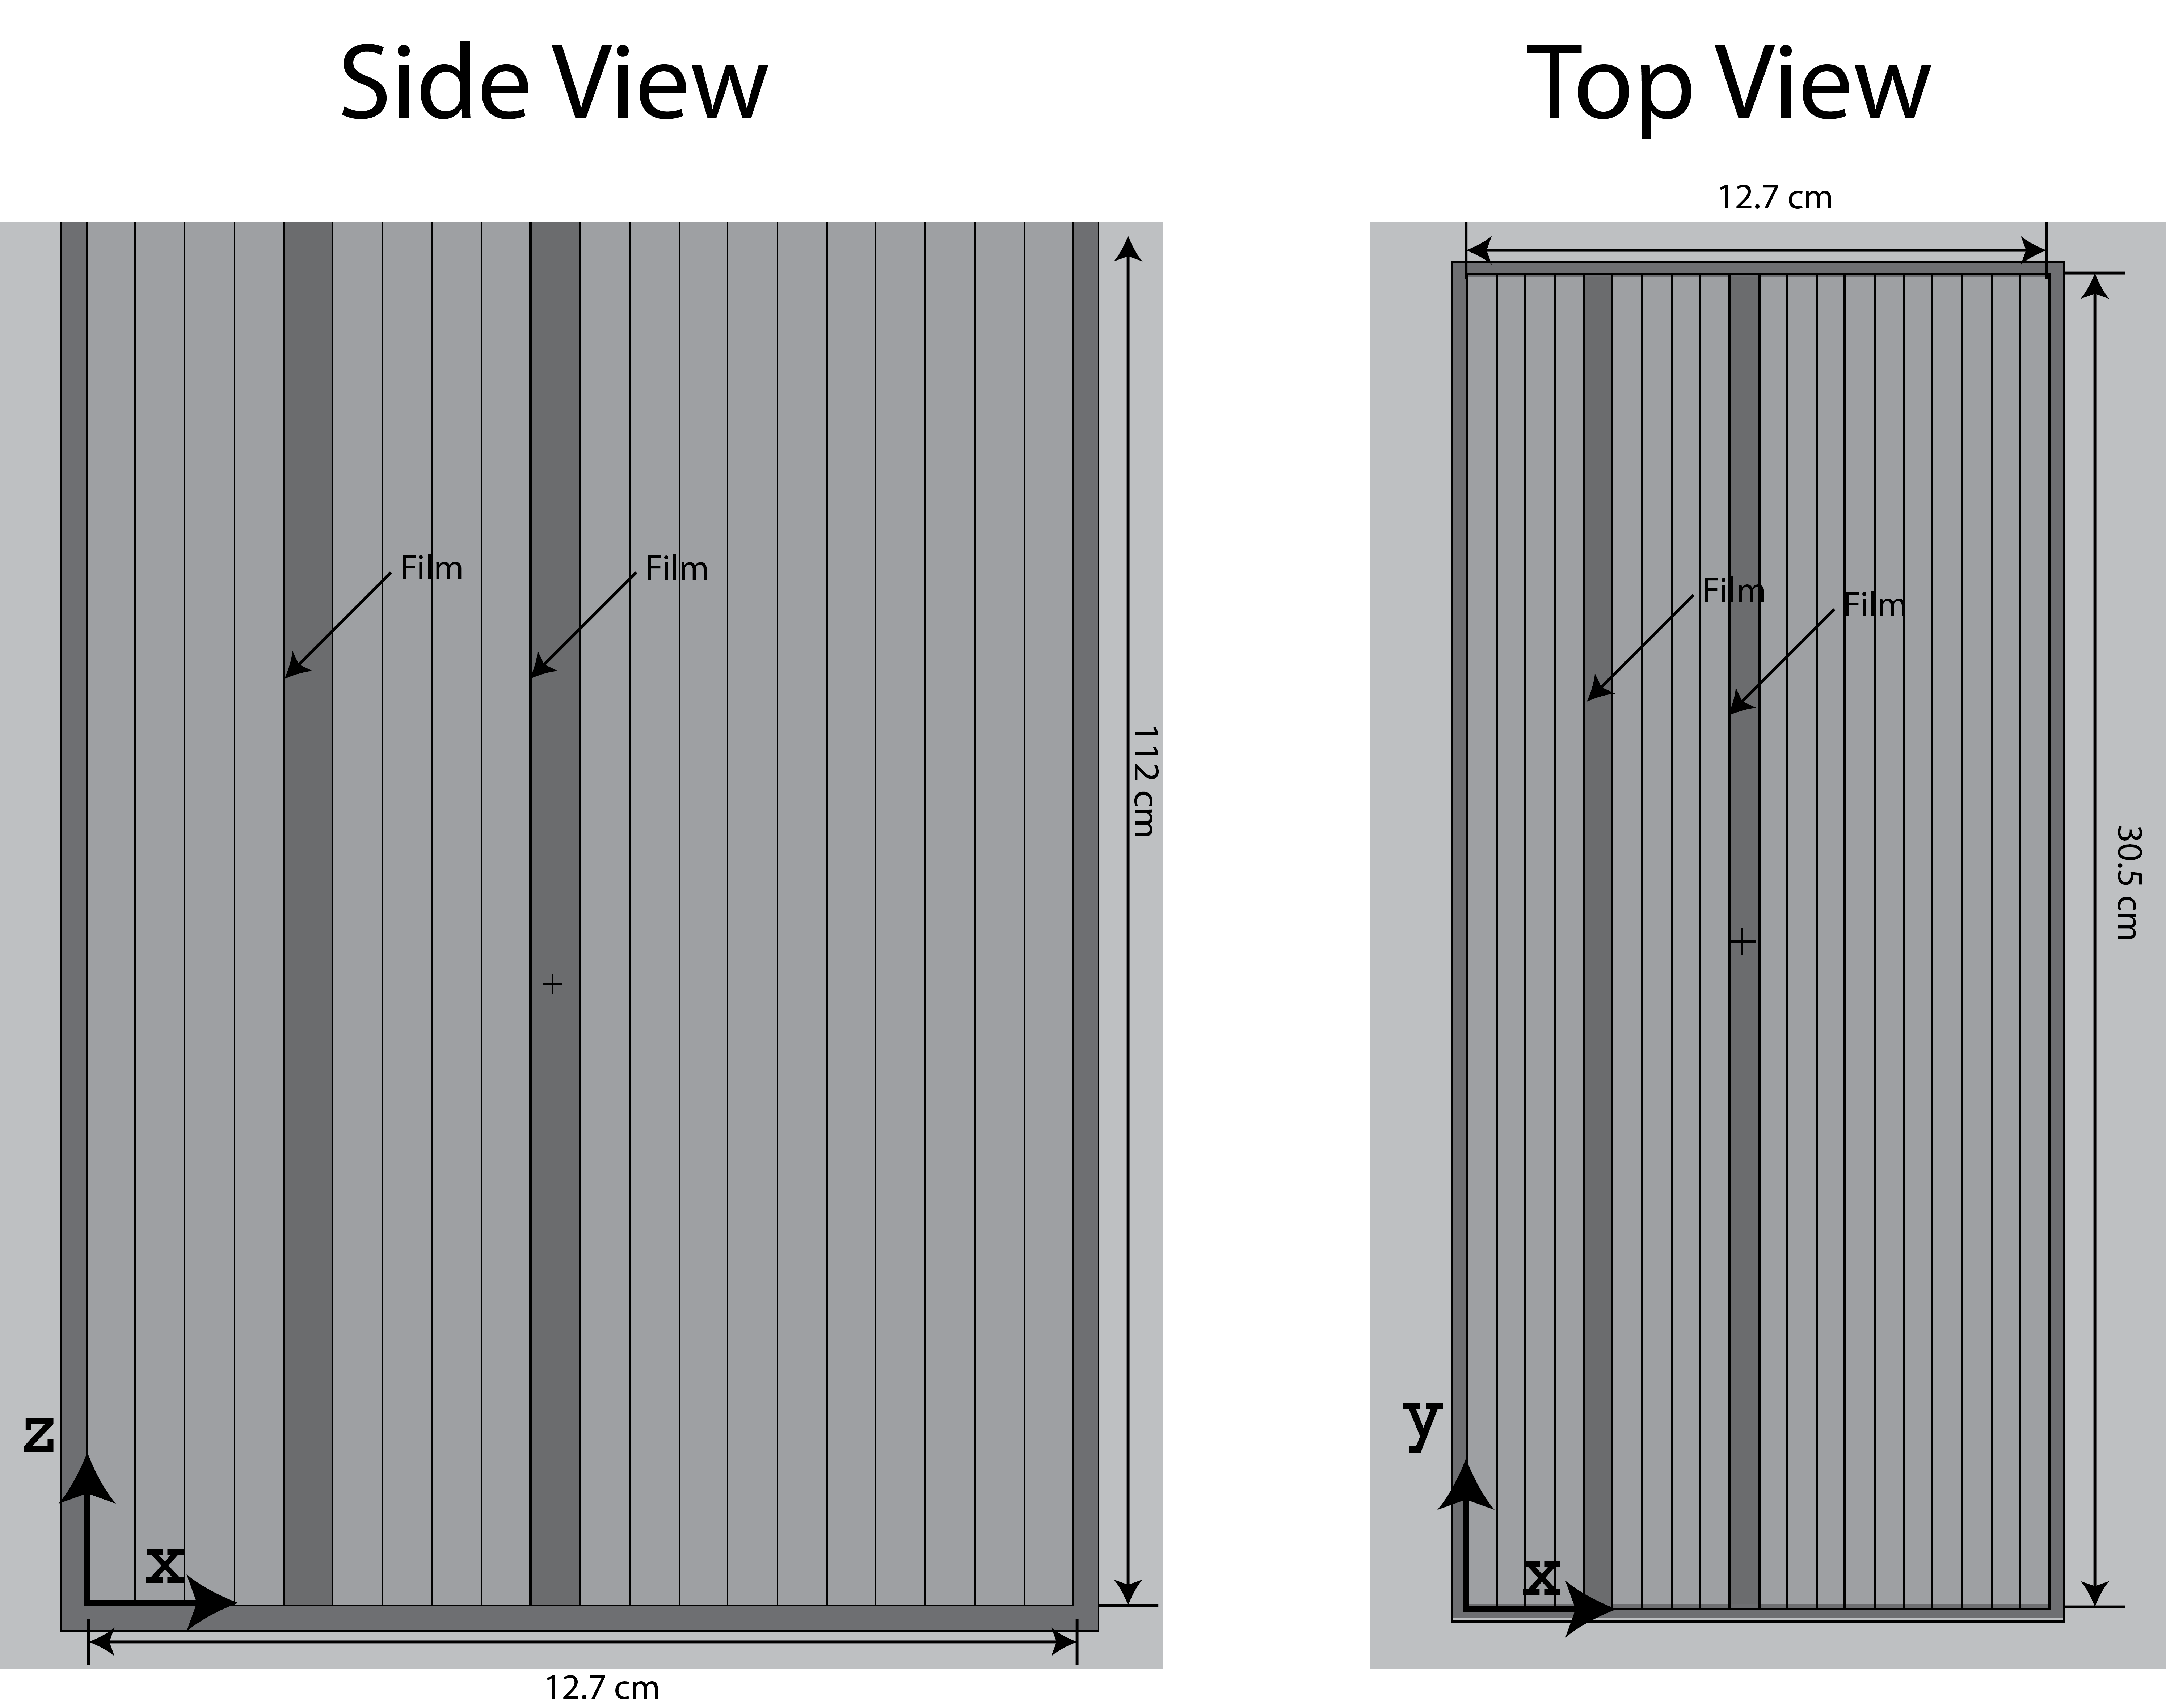
\includegraphics[width=\textwidth]{RPM8OptLayered_LiFZnSBW}
  \caption[]{Example geometry of a film inside the radiation portal monitor. The film material is \iso[6]{LiF} loaded ZnS:Ag, which has a high loading of \iso[6]{Li}. The origin is shown in the lower left of each figure, along with the axis.}
  \label{fig:EXSumDemoLiFZnS}
\end{figure}

The positions of the films necessary to meet the detector criteria are shown in \autoref{tab:EXSumPerf}.
These layered detector designs consist of \SI{100}{\um}, \iso[6]{Li} fluoride loaded polymers that are encased in \SI{5}{\mm} of a wavelength shifting plastic in addition to a \SI{100}{\um} \iso[6]{LiF} loaded ZnS:Ag commercial scintillator also encased in a wavelength shifter.
The wavelength shifter was assumed to have a material composition similar to that of high density polyethylene, which also served as the moderator.
In the case of the polyethylene naphthalene film an alternative method of neutron - gamma discrimination shows promise in which the entire neutron spectra can be utilized. 
In this case only two detector films are necessary, spaced at \SI{2.54}{\cm} and \SI{5.08}{\cm}.
In addition to layered designs a design in which the \iso[6]{Li} detector layers are wrapped around into concentric cylinders was also explored. 
A design using four cylinders (each 2 cm in outer diameter) placed equidistant in the RPM8 loaded with 30\% \iso[6]{Li} fluoride (using \SI{28}{\g} of \iso[6]{Li}) would have an interaction rate above 3.2 interactions per second per nanogram \iso[252]{Cf}.
If two photomultiplier tubes are placed at the top and bottom of a fishtail light guide mounted on the top and bottom of the detector cabinet, eight percent of the optical photons generated in a 10 percent loaded polystyrene film can be collected, leaving 160 photons to produce a signal on the photomultiplier tubes.
\begin{table}
  \caption[]{Simulated detector performance in a design capable of meeting the DHS / DNDO criteria.}
  \label{tab:EXSumPerf}
  \begin{tabular}{m{5cm} m{5cm} m{3cm}}
    \toprule
    Detector Composition & Film Positions & Expected Photons Collected \\
    \midrule
    10\% \iso[6]{LiF} polystyrene & \SI{2.54}{\cm}, \SI{3.82}{\cm}, \SI{6.36}{\cm} & 160 \\
    10\% \iso[6]{LiF} polyethylene naphthalene & \SI{1.90}{\cm}, \SI{3.82}{\cm}, \SI{5.08}{\cm} & 240 \\
    \iso[6]{LiF} loaded ZnS:Ag &\SI{3.17}{\cm}, \SI{6.35}{\cm} & 1,900\\
    \bottomrule
  \end{tabular}
\end{table}

 
